\documentclass[unicode,11pt,a4paper,oneside,numbers=endperiod,openany]{scrartcl}

\usepackage{ifthen}
\usepackage[utf8]{inputenc}
\usepackage{graphics}
\usepackage{graphicx}
\usepackage{hyperref}

\pagestyle{plain}
\voffset -5mm
\oddsidemargin  0mm
\evensidemargin -11mm
\marginparwidth 2cm
\marginparsep 0pt
\topmargin 0mm
\headheight 0pt
\headsep 0pt
\topskip 0pt        
\textheight 255mm
\textwidth 165mm

\newcommand{\duedate} {}
\newcommand{\setduedate}[1]{%
\renewcommand\duedate {See iCorsi for due date}}
\newcommand\isassignment {false}
\newcommand{\setassignment}{\renewcommand\isassignment {true}}
\newcommand{\ifassignment}[1]{\ifthenelse{\boolean{\isassignment}}{#1}{}}
\newcommand{\ifnotassignment}[1]{\ifthenelse{\boolean{\isassignment}}{}{#1}}

\newcommand{\assignmentpolicy}{
\begin{table}[h]
\begin{center}
\scalebox{0.8} {%
\begin{tabular}{|p{0.02cm}p{16cm}|}
\hline
&\\
\multicolumn{2}{|c|}{\Large\textbf{HPC Lab ---  Submission Instructions}}\\
\multicolumn{2}{|c|}{\large\textbf{(Please, notice that following instructions are mandatory: }}\\
\multicolumn{2}{|c|}{\large\textbf{submissions that don't comply with, won't be considered)}}\\
&\\
\textbullet & Assignments must be submitted to \href{https://www.icorsi.ch}{iCorsi} (i.e. in electronic format).\\
\textbullet & Provide both executable package and sources (e.g. C/C++ files, Matlab). 
If you are using libraries, please add them in the file. Sources must be organized in directories called:\\
\multicolumn{2}{|c|}{\textit{Project\_number\_lastname\_firstname}}\\
& and  the  file must be called:\\
\multicolumn{2}{|c|}{\textit{project\_number\_lastname\_firstname.zip}}\\
\multicolumn{2}{|c|}{\textit{project\_number\_lastname\_firstname.pdf}}\\
\textbullet &  The TAs will grade your project by reviewing your project write-up, and looking at the implementation 
                 you attempted, and benchmarking your code's performance.\\

\textbullet & You are allowed to discuss all questions with anyone you like; however: (i) your submission must list anyone you discussed problems with and (ii) you must write up your submission independently.\\
\hline
\end{tabular}
}
\end{center}
\end{table}
}
\newcommand{\punkte}[1]{\hspace{1ex}\emph{\mdseries\hfill(#1~\ifcase#1{Points}\or{Points}\else{Points}\fi)}}


\newcommand\serieheader[6]{
\thispagestyle{empty}%
\begin{flushleft}

\includegraphics[width=0.4\textwidth]{media/usi_inf.png}
\end{flushleft}
  \noindent%
  {\large\ignorespaces{\textbf{#1}}\hspace{\fill}\ignorespaces{ \textbf{#2}}}\\ \\%
  {\large\ignorespaces #3 \hspace{\fill}\ignorespaces #4}\\
  \noindent%
  \bigskip
  \hrule\par\bigskip\noindent%
  \bigskip {\ignorespaces {\Large{\textbf{#5}}}
  \hspace{\fill}\ignorespaces \large \ifthenelse{\boolean{\isassignment}}{\duedate}{#6}}
  \hrule\par\bigskip\noindent%  \linebreak
 }

\makeatletter
\def\enumerateMod{\ifnum \@enumdepth >3 \@toodeep\else
      \advance\@enumdepth \@ne
      \edef\@enumctr{enum\romannumeral\the\@enumdepth}\list
      {\csname label\@enumctr\endcsname}{\usecounter
        {\@enumctr}%%%? the following differs from "enumerate"
	\topsep0pt%
	\partopsep0pt%
	\itemsep0pt%
	\def\makelabel##1{\hss\llap{##1}}}\fi}
\let\endenumerateMod =\endlist
\makeatother




\usepackage{textcomp}





\usepackage{ntheorem}
\usepackage{subcaption}
\usepackage{booktabs}
\usepackage{multirow}
\usepackage{tabularx}
\usepackage{listings}
\usepackage{amsmath}
\usepackage{graphicx}
\usepackage{float}
\usepackage[dvipsnames]{xcolor}
\usepackage[
	backend=biber,
]{biblatex}
\addbibresource{bib/sources.bib}
\theoremstyle{plain}
\theorembodyfont{\upshape} % or "\itshape", or whatever
\newtheorem{question}{Question}

\definecolor{codegreen}{rgb}{0,0.6,0}
\definecolor{codegray}{rgb}{0.5,0.5,0.5}
\definecolor{codepurple}{rgb}{0.58,0,0.82}
\definecolor{codeblue}{rgb}{0.251, 0.471, 0.753}
\definecolor{backcolour}{rgb}{0.961, 0.961, 0.961}

\lstdefinestyle{mystyle}{%
    backgroundcolor=\color{backcolour},   
    commentstyle=\color{Fuchsia}\textit,
    keywordstyle=\color{NavyBlue},
    numberstyle=\tiny\color{codegray},
    stringstyle=\color{Green},
    basicstyle=\ttfamily\footnotesize,
    breakatwhitespace=false,         
    breaklines=true,                 
    captionpos=b,                    
    keepspaces=true,                 
    numbers=left,                    
    numbersep=5pt,                  
    showspaces=false,                
    showstringspaces=false,
    showtabs=false,                  
    tabsize=2,
}


\lstset{style=mystyle}

\begin{document}

\setassignment

\serieheader{High-Performance Computing Lab}{Institute of Computing}{Student: Dennys Mike Huber}{Discussed with: Alberto Finardi \& Leon Ackermann}{Solution for Project 3}{}
\newline
This project will introduce you a parallel space solution of a nonlinear PDE using OpenMP.
\section{Implementing the linear algebra functions and the stencil operators [35 Points]}
After implementing the missing functions and the stencil kernel, given by the formula \ref{eq:stencil}, the serial code produces the output seen in Subfigure \ref{fig:serial}, which is approximately the same as the provided reference output in the project description.
\begin{equation} \label{eq:stencil}
f_{i, j}^k=\left[-(4+\alpha) s_{i, j}^k+s_{i-1, j}^k+s_{i+1, j}^k+s_{i, j-1}^k+s_{i, j+1}^k+\beta s_{i, j}^k\left(1-s_{i, j}^k\right)\right]+\alpha s_{i, j}^{k-1}
\end{equation}
Furthermore the resulting population concentration at final time is depicted in Subfigure \ref{fig:output_serial}.
\begin{figure}[H]
    \centering
    \begin{subfigure}[b]{0.6\textwidth}
        \centering
	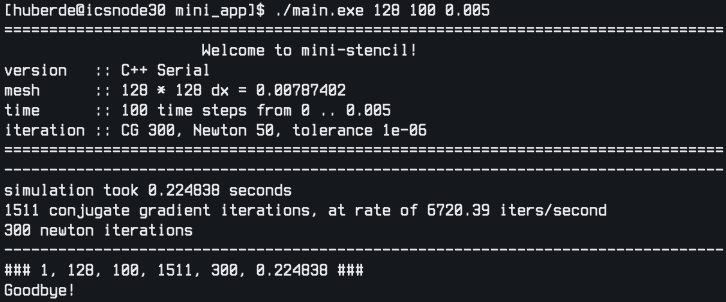
\includegraphics[width=\textwidth]{../media/serial_output.png}
	\caption{Output after implementing the linear algebra function and stencil operators.}
	\label{fig:serial}
    \end{subfigure}
    \hfill 
    \begin{subfigure}[b]{0.39\textwidth}
        \centering
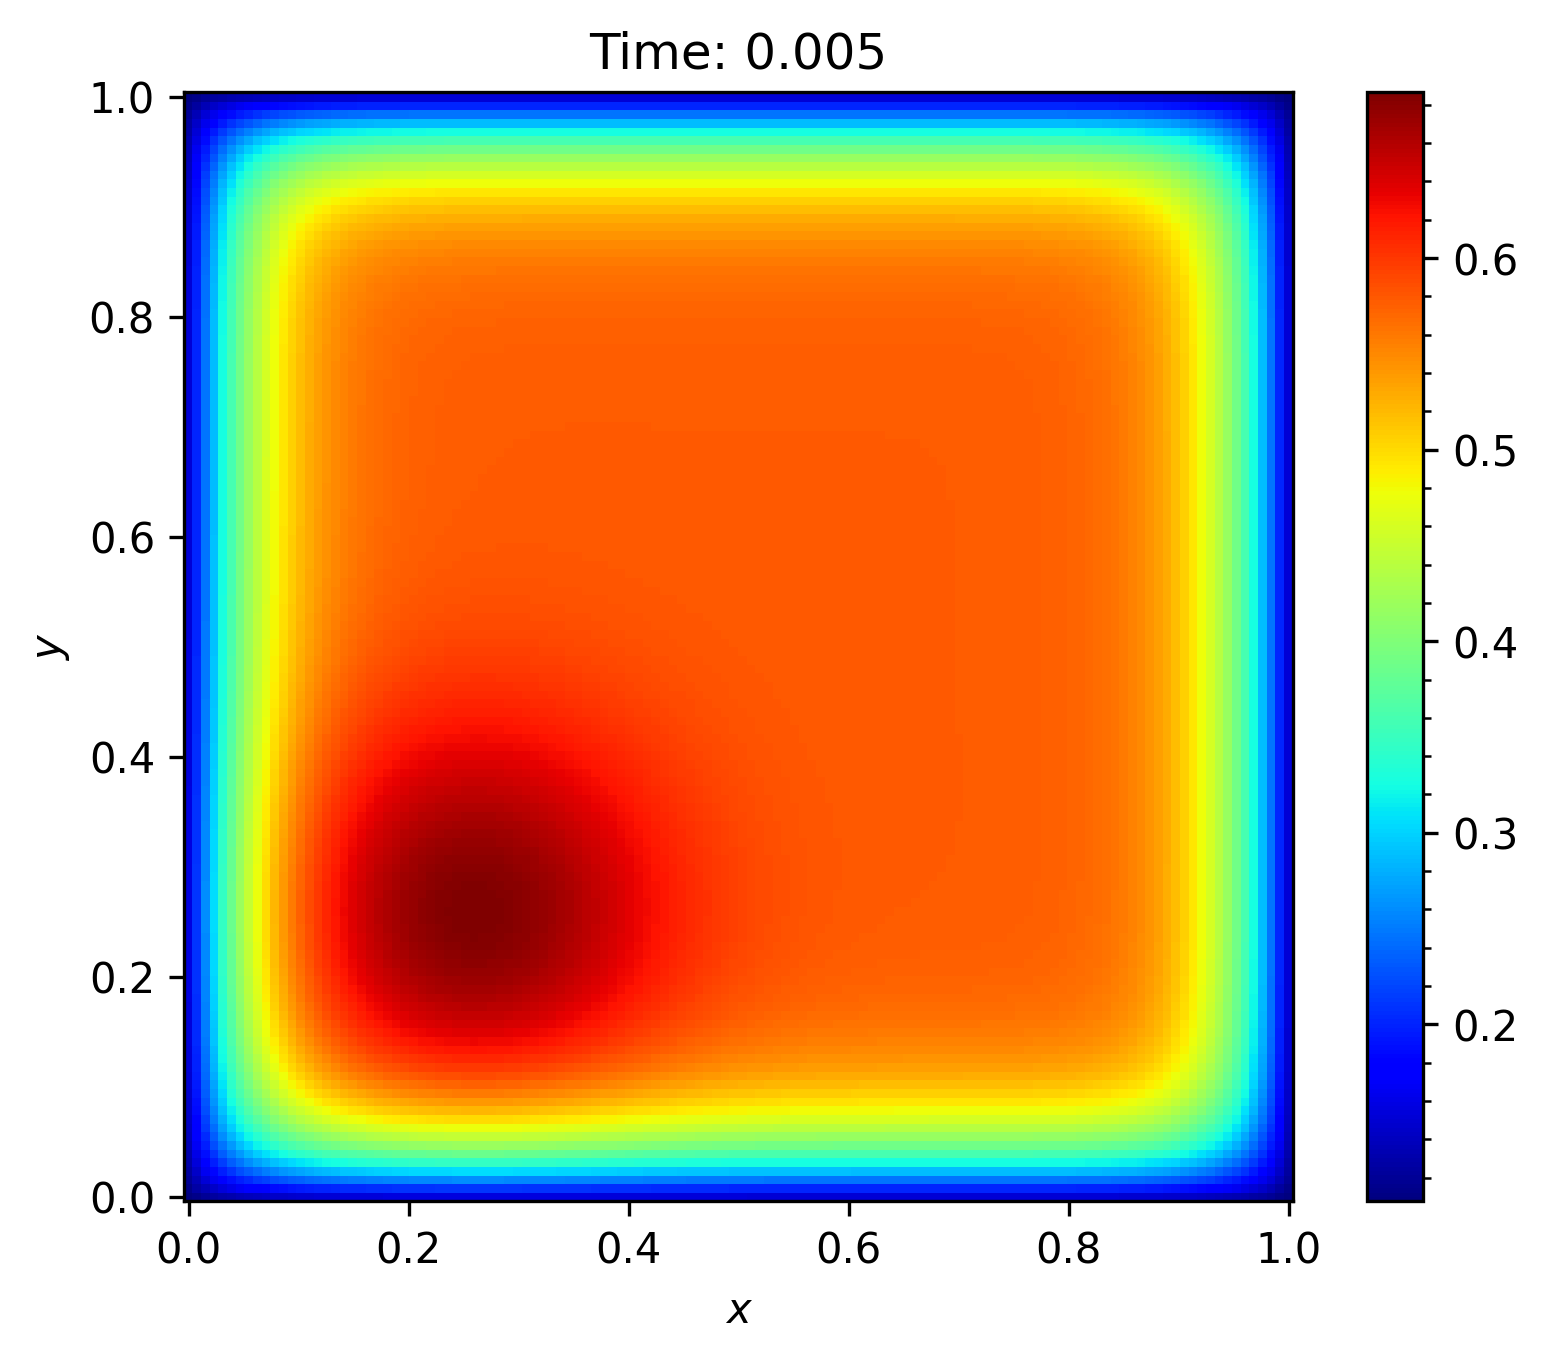
\includegraphics[width=\textwidth]{../media/output_serial.png}
	\caption{Population concentration at $t=0.005$.}
	\label{fig:output_serial}

    \end{subfigure}
    \caption{Results of the Mini App, when implemented in serial.}
    \label{fig:mini_app}
\end{figure}

\section{Adding OpenMP to the nonlinear PDE mini-app [50 Points]}

\subsection{Implementation}
In order to ensure that the mini-app still compiles without OpenMP enabled we introduce the following macro
\begin{lstlisting}[language=C++, caption=\_OpenMP macro, label=lst:omp-macro]
#ifdef _OPENMP
/* CODE */
#else
/* CODE */
#endif
\end{lstlisting}
which functions similar to an \texttt{if} statement, that is evaluated at compile time.
All the necessary functions from the OpenMP that would conflict with the compilation process (which does not include the \texttt{\#pragma omp} statements) are placed inside the \texttt{\#ifdef} macro. \cite{noauthor_conditional_nodate}
The updated welcome massage can be seen in Figure \ref{fig:welcome}
\begin{figure}[H]
	\centering
	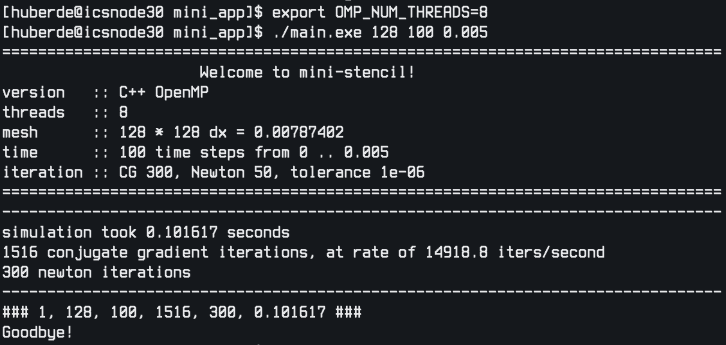
\includegraphics[width=0.8\textwidth]{../media/welcome_parallel.png}
	\caption{Welcome Massage for parallel Implementation}
	\label{fig:welcome}
\end{figure}
For the parallelization of all the loops in the \texttt{linalg.c} file, I introduce basic OpenMP pragma for loops statements including the reduction clause, when necessary. No extra clauses were introduced, because these are rather simple loops, which OpenMP should be able to optimize very well on its own.\newline
\newline
In contrast for the diffusion stencil different ways of optimizing the loop were experimented on. This included using the \texttt{collapse} clause for the inner grid points \cite{noauthor_collapse_nodate}, trying out different loop scheduling (static, guided, dynamic), as well as parallelizing the loops for the boundary points. None of these approaches brought a significant improvement to the execution, therefore the decision was taken to resort to the simplest solution, which is simply to use \texttt{\#pragma omp parallel for} statement for the inner grid points and let OpenMP do all the optimization.

\subsection{Boundary Loops}
The boundary loops play a essential role in diffusion simulations by appropriately handling boundary conditions. By enforcing boundary conditions they are maintaining the stability and correctness of the model. In the mini-app they are split up in East, West, North, South and Corners. Each boundary loop has a unique constraint that needs to taken into consideration, this includes handling points outside of the domain or including fixed boundary values.



\subsection{Bitwise identical results}
Producing a bitwise-identical result using more than one thread in OpenMP can be a challenge, because of the non-associativity of floating point addition or multiplications, which can lead to different results even when using the same number of threads. More specifically when using the reduction clause, OpenMP does not specify the location nor the order in which the values are combined. This can lead to different rounding errors, due to the limited accuracy of floating point operations, depending on the order of the reduction \cite{noauthor_reduction_nodate}. Technically it would be possible to have bitwise-identical solution for a fixed number of threads, where we guarantee that always the same chunk of data is processed by a thread and then have a fixed order in which we reduce individual results, but as soon as we change the number of threads we can not guarantee a bitwise-identical solution. In addition this method would have a clear impact on performance, because these additional assumption we would need to take would create an additional overhead.

\subsection{Strong \& Weak Scaling Analysis}
In the strong analysis scenario, where the problem size is constant and the goal is to reduce the execution time by increasing the number of threads. The Figure \ref{fig:strong} depicts the execution time in seconds versus the number of threads, for the y-axis a logarithmic scale was chosen in order to examine the variations in timing across different resolutions.\newline
For the smallest problem size in $N=64\times64$ the curve is basically flat for 2 to 4 number of threads, increasing it even further the execution time starts to increase, which is caused by the increasing overhead created by OpenMP, when handling synchronization, communication and thread management. This clearly outweighs the benefits given by the parallelization. This behavior clearly indicates that for efficient use of the threads the work load is too small. Increasing the resolution, we can now clearly see a reduction of execution from threads 2 to 4 for the $N=128 \times 128$ and even from threads 2 to 8 for the resolutions from $N=256\times256$ to $N=1024\times1024$. This clearly shows that all these resolution benefit from a increasing number of threads, yet when increasing to 16 threads for all the resolution the execution time increases or stays relatively stable (for higher resolutions). This is again caused by the increasing overhead. In addition this clearly shows that for all resolution a saturation point is reached, after which the benefits diminish. \newline
\newline
In the weak scaling scenario, when increasing the number of threads, the workload per thread stays constant. In the optimal scenario the execution time stays constant, when scaling up the number of threads and resolution. This resolution is adjusted by the following formula
\begin{equation}
	n = n_{\text{base}} \cdot \sqrt{N_{\text{CPU}}}
\end{equation}
If there is an increase in execution time this represents the overhead created by the communication, thread management and synchronization. The results of the mini-app using weak scaling can be seen in Figure \ref{fig:weak}, where a logarithmic scale was used for the y-axis to compare the execution times more conveniently. In addition the dashed lines indicate the constant optimal execution time. Smaller base resolutions ($64 \times 64$ and $128\times128$) clearly show less efficient weak scaling. For smaller number of threads the execution time increases significantly. Once more this shows the overhead encountered is substantial in comparison to the workload. This suggests that problem size might be too small to leverage parallel resources more effectively. For higher base resolution ($256 \times 256$) weak scaling is improved, which can be seen by the more gradual grow when increasing the number of threads, suggesting that due to the higher resolutions the overhead is less dominant. When comparing curves for each base resolution to its optimal weak scaling, we can clearly make out a strong deviation, which becomes more noticeable when increasing the number of threads and as a consequence, also the overhead.

\begin{figure}[H]
    \centering
    \begin{subfigure}[b]{0.8\textwidth}
        \centering
	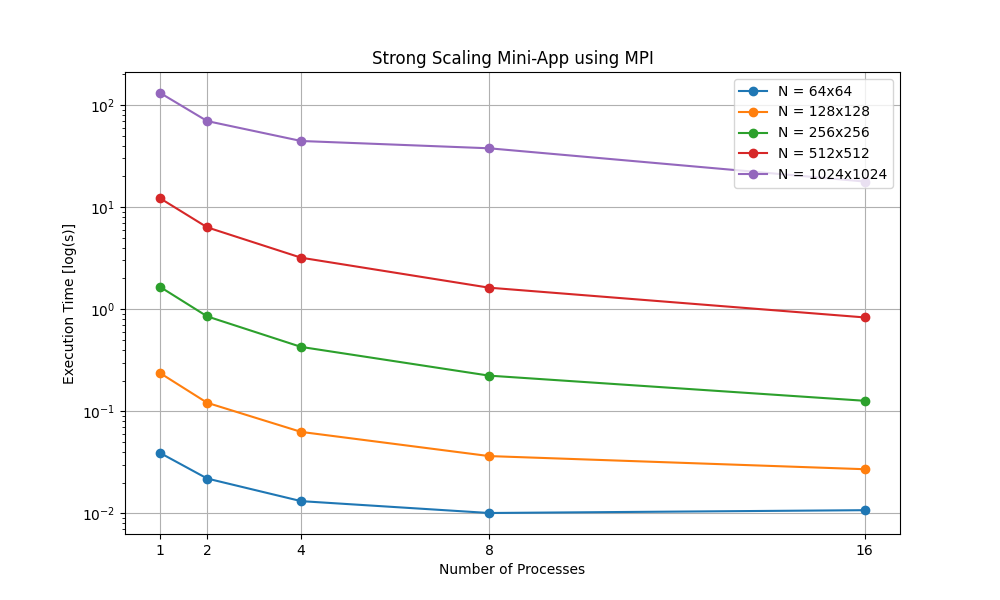
\includegraphics[width=\textwidth]{../media/strong_scaling.png}
	\caption{Strong Scaling}
	\label{fig:strong}
    \end{subfigure}
    \hfill 
    \begin{subfigure}[b]{0.8\textwidth}
        \centering
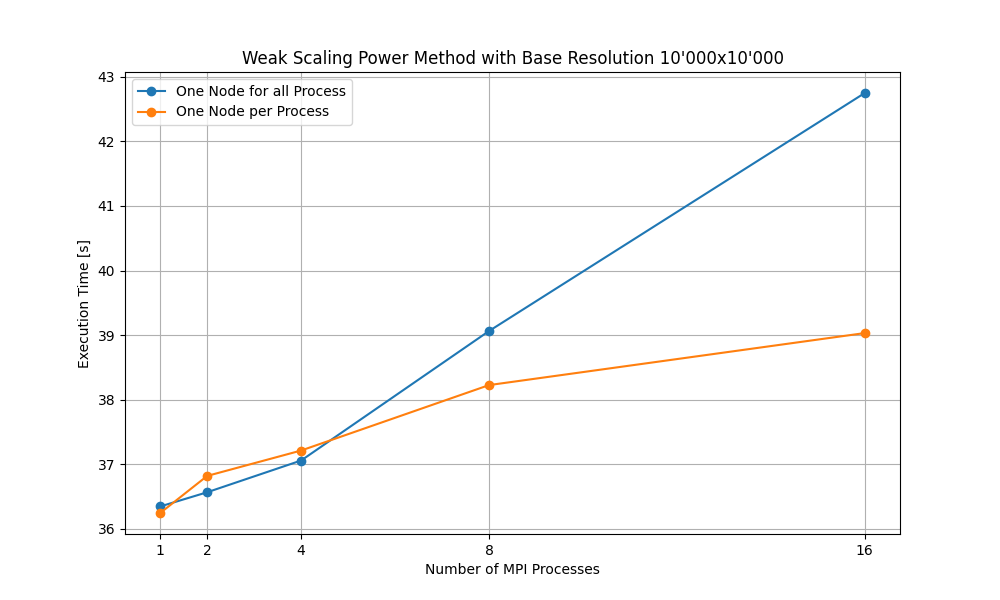
\includegraphics[width=\textwidth]{../media/weak_scaling.png}
	\caption{Weak Scaling}
	\label{fig:weak}

    \end{subfigure}
    \caption{Scaling Plots of the mini-app}
    \label{fig:scaling}
\end{figure}



% \newpage
\printbibliography[heading=bibintoc]
\end{document}
